
\subsection{Background segmentation}

The background segmentation node is based on the backgroundSubtractorMOG2 from OpenCV \cite{BGS} which uses Gaussian mixtures to perform the segmentation. The background segmentation results in a binary image of the foreground. The background modeling uses statistical properties by model each pixel as a mixture of gaussian. A pixel is counted as foreground when it deviates from these gaussians. Checking each pixel in the fram gives out the entire foreground. The background model updates for each frame processed which means it is computationally expensive. 

\begin{figure}[H]
\begin{center}
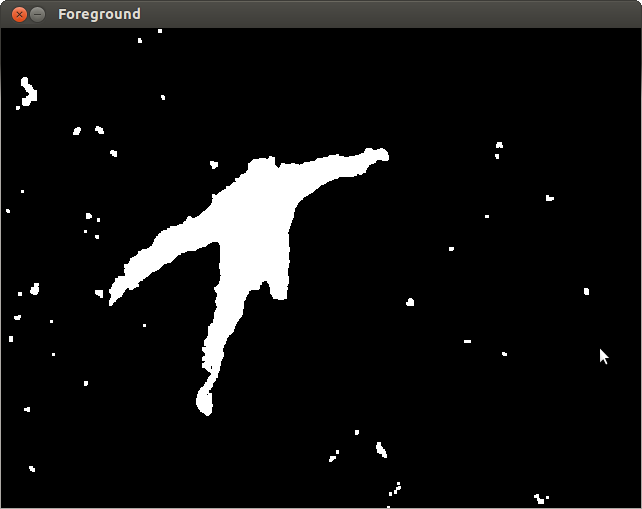
\includegraphics[width=12 cm]{screenshot_foreground_image}
\caption{Foreground from background segmentation}

\end{center}
\end{figure}


The foreground and depth image are used to construct a point cloud. For each foreground pixel the corresponding depth value $Z$, pixel coordinates $x$, $y$ and intrinsic parameter can be used to obtain the world coordinates as follows.

\begin{center}
$\displaystyle X = (x - c_x) \cdot \frac{Z}{f_x}$\\ \vspace{10 pt}
$\displaystyle Y = (y - c_y) \cdot \frac{Z}{f_y}$

and the 3D point is ${\bf P} = [X, Y, Z]^T$
\end{center}


By applying these formulas to all foreground pixels the point cloud is obtained.


